% Options for packages loaded elsewhere
\PassOptionsToPackage{unicode}{hyperref}
\PassOptionsToPackage{hyphens}{url}
%
\documentclass[
]{book}
\usepackage{lmodern}
\usepackage{amssymb,amsmath}
\usepackage{ifxetex,ifluatex}
\ifnum 0\ifxetex 1\fi\ifluatex 1\fi=0 % if pdftex
  \usepackage[T1]{fontenc}
  \usepackage[utf8]{inputenc}
  \usepackage{textcomp} % provide euro and other symbols
\else % if luatex or xetex
  \usepackage{unicode-math}
  \defaultfontfeatures{Scale=MatchLowercase}
  \defaultfontfeatures[\rmfamily]{Ligatures=TeX,Scale=1}
\fi
% Use upquote if available, for straight quotes in verbatim environments
\IfFileExists{upquote.sty}{\usepackage{upquote}}{}
\IfFileExists{microtype.sty}{% use microtype if available
  \usepackage[]{microtype}
  \UseMicrotypeSet[protrusion]{basicmath} % disable protrusion for tt fonts
}{}
\makeatletter
\@ifundefined{KOMAClassName}{% if non-KOMA class
  \IfFileExists{parskip.sty}{%
    \usepackage{parskip}
  }{% else
    \setlength{\parindent}{0pt}
    \setlength{\parskip}{6pt plus 2pt minus 1pt}}
}{% if KOMA class
  \KOMAoptions{parskip=half}}
\makeatother
\usepackage{xcolor}
\IfFileExists{xurl.sty}{\usepackage{xurl}}{} % add URL line breaks if available
\IfFileExists{bookmark.sty}{\usepackage{bookmark}}{\usepackage{hyperref}}
\hypersetup{
  pdftitle={Screen Pixel Ruler {[}master{]}},
  pdfauthor={Stewart Cossey},
  hidelinks,
  pdfcreator={LaTeX via pandoc}}
\urlstyle{same} % disable monospaced font for URLs
\usepackage{longtable,booktabs}
% Correct order of tables after \paragraph or \subparagraph
\usepackage{etoolbox}
\makeatletter
\patchcmd\longtable{\par}{\if@noskipsec\mbox{}\fi\par}{}{}
\makeatother
% Allow footnotes in longtable head/foot
\IfFileExists{footnotehyper.sty}{\usepackage{footnotehyper}}{\usepackage{footnote}}
\makesavenoteenv{longtable}
\usepackage{graphicx,grffile}
\makeatletter
\def\maxwidth{\ifdim\Gin@nat@width>\linewidth\linewidth\else\Gin@nat@width\fi}
\def\maxheight{\ifdim\Gin@nat@height>\textheight\textheight\else\Gin@nat@height\fi}
\makeatother
% Scale images if necessary, so that they will not overflow the page
% margins by default, and it is still possible to overwrite the defaults
% using explicit options in \includegraphics[width, height, ...]{}
\setkeys{Gin}{width=\maxwidth,height=\maxheight,keepaspectratio}
% Set default figure placement to htbp
\makeatletter
\def\fps@figure{htbp}
\makeatother
\setlength{\emergencystretch}{3em} % prevent overfull lines
\providecommand{\tightlist}{%
  \setlength{\itemsep}{0pt}\setlength{\parskip}{0pt}}
\setcounter{secnumdepth}{-\maxdimen} % remove section numbering
\usepackage{booktabs}
\usepackage{amsthm}
\makeatletter
\def\thm@space@setup{%
  \thm@preskip=8pt plus 2pt minus 4pt
  \thm@postskip=\thm@preskip
}
\makeatother
\usepackage[]{natbib}
\bibliographystyle{plainnat}

\title{Screen Pixel Ruler {[}master{]}}
\author{Stewart Cossey}
\date{2021-12-04}

\begin{document}
\maketitle

{
\setcounter{tocdepth}{1}
\tableofcontents
}
\hypertarget{overview}{%
\chapter{Overview}\label{overview}}

Screen Pixel Ruler is a on screen ruler that can assist in measuring elements from web pages, documents or software which does not implement a native ruler.
Based on .NET Core 3.1 and inspired by MioPlanet PixelRuler.

\hypertarget{features}{%
\section{Features}\label{features}}

\begin{itemize}
\tightlist
\item
  Global hotkeys to trigger functionality when other software is in focus.
\item
  Rotatable vertical or horizontal ruler. \emph{Ctrl + Shift + Alt + R}
\item
  Customizable ruler themes.
\item
  Freezable position. \emph{Ctrl + Shift + Alt + F}
\item
  Guideline system that can lock the mouse cursor horizontally or vertically
\item
  Position 0 of the ruler to the current cursor location. \emph{Ctrl + Shift + Alt + S}
\end{itemize}

\hypertarget{ui}{%
\chapter{User Interface}\label{ui}}

The user interface consists of a single ruler that can be displayed either horizontally or vertically.

\begin{figure}
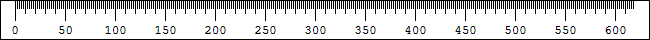
\includegraphics[width=1\linewidth]{images/ruler} \caption{The Ruler user interface.}\label{fig:unnamed-chunk-1}
\end{figure}

\hypertarget{guidelines}{%
\chapter{Guidelines}\label{guidelines}}

Guidelines allow you to mark specific points on the ruler.

\hypertarget{adding-and-removing-guidelines}{%
\section{Adding and Removing Guidelines}\label{adding-and-removing-guidelines}}

You can add and remove guidelines by using the Ruler Menu \textgreater{} Guidelines submenu.

Adding a guideline will add it in positio

\hypertarget{clearing-guidelines}{%
\section{Clearing Guidelines}\label{clearing-guidelines}}

\hypertarget{importing-and-exporting-guidelines}{%
\section{Importing and Exporting Guidelines}\label{importing-and-exporting-guidelines}}

\hypertarget{keyboard}{%
\chapter{Global Shortcuts}\label{keyboard}}

These shortcuts can be used even when the Screen Pixel Ruler is not focused.

\begin{longtable}[]{@{}ll@{}}
\toprule
\begin{minipage}[b]{0.27\columnwidth}\raggedright
Keystroke\strut
\end{minipage} & \begin{minipage}[b]{0.68\columnwidth}\raggedright
Function\strut
\end{minipage}\tabularnewline
\midrule
\endhead
\begin{minipage}[t]{0.27\columnwidth}\raggedright
Ctrl + Shift + Alt + R\strut
\end{minipage} & \begin{minipage}[t]{0.68\columnwidth}\raggedright
Change ruler rotation.\strut
\end{minipage}\tabularnewline
\begin{minipage}[t]{0.27\columnwidth}\raggedright
Ctrl + Shift + Alt + E\strut
\end{minipage} & \begin{minipage}[t]{0.68\columnwidth}\raggedright
Flip ruler notch direction.\strut
\end{minipage}\tabularnewline
\begin{minipage}[t]{0.27\columnwidth}\raggedright
Ctrl + Shift + Alt + F\strut
\end{minipage} & \begin{minipage}[t]{0.68\columnwidth}\raggedright
Freeze the position marker on the ruler.\strut
\end{minipage}\tabularnewline
\begin{minipage}[t]{0.27\columnwidth}\raggedright
Ctrl + Shift + Alt + S\strut
\end{minipage} & \begin{minipage}[t]{0.68\columnwidth}\raggedright
Move position 0 of the ruler to the current mouse position.\strut
\end{minipage}\tabularnewline
\begin{minipage}[t]{0.27\columnwidth}\raggedright
Ctrl + Shift + Alt + X\strut
\end{minipage} & \begin{minipage}[t]{0.68\columnwidth}\raggedright
Exit Screen Pixel Ruler 2.\strut
\end{minipage}\tabularnewline
\begin{minipage}[t]{0.27\columnwidth}\raggedright
Ctrl + Shift + Alt + A\strut
\end{minipage} & \begin{minipage}[t]{0.68\columnwidth}\raggedright
Add Guideline at current position on the ruler.\strut
\end{minipage}\tabularnewline
\begin{minipage}[t]{0.27\columnwidth}\raggedright
Ctrl + Shift + Alt + D\strut
\end{minipage} & \begin{minipage}[t]{0.68\columnwidth}\raggedright
Delete nearest Guideline from current position on the ruler.\strut
\end{minipage}\tabularnewline
\begin{minipage}[t]{0.27\columnwidth}\raggedright
Ctrl + Shift + Alt + G\strut
\end{minipage} & \begin{minipage}[t]{0.68\columnwidth}\raggedright
Lock mouse position to nearest Guideline.\strut
\end{minipage}\tabularnewline
\bottomrule
\end{longtable}

\hypertarget{config}{%
\chapter{Configuration}\label{config}}

You can access the configuration by right clicking the ruler and selecting \emph{Options}.
This will then display the \emph{Options window} where you can change the configuration.

\hypertarget{options}{%
\section{Options}\label{options}}

Theme\\
Allows you to change the \protect\hyperlink{themes}{theme} of the ruler.

\hypertarget{location}{%
\section{Location}\label{location}}

Configuration is stored in two locations depending on if you installed from the installer or from the chocolatey package.
Configuration is in \emph{yaml}.

Installer: \%appdata\%\textbackslash screenpixelruler\textbackslash app.cfg\\
Chocolatey: \%chocolateyinstall\%\textbackslash lib\textbackslash screenpixelruler\textbackslash tools\textbackslash app.cfg

\hypertarget{themes}{%
\chapter{Themes}\label{themes}}

Themes can change the ruler colour, size or even the size of the ruler notches.

You can create your own themes for Screen Pixel Ruler.
Themes have a \texttt{thm} file extension and are writtem in \emph{yaml}.

\hypertarget{location-1}{%
\section{Location}\label{location-1}}

Themes are stored in the two locations, depending on if you installed from the installer or from the chocolatey package.

Installer: \%appdata\%\textbackslash screenpixelruler\\
Chocolatey: \%chocolateyinstall\%\textbackslash lib\textbackslash screenpixelruler\textbackslash tools

\end{document}
